% Preamble
% ---
\documentclass{article}

% Packages

% \usepackage{graphicx}
% \usepackage{subfig}

\usepackage{multicol}
\usepackage{float}

\usepackage{tikz}
\usepackage{pgfplots}
\usepgfplotslibrary{external}
% \usetikzlibrary{shapes.geometric, arrows}
% 
\usepackage[english]{babel}

\usepackage{geometry}
\geometry{margin=1.2cm}

% ---

% \graphicspath{ {assets/} }

% \setlength{\columnsep}{1.3cm}

% \setlength{\columnsep}{0.8cm}
\begin{document}
\begin{multicols}{2}

\section{Introduction}

\section{Serial Optimisation}

\subsection{Reduce Memory Accesses}
In the original implementation of the algorithm for each timestep the
\verb|cells| array was looped over the 4 times, in \verb|propagate|,
\verb|rebound|, \verb|collision| and \verb|av_velocity|. This resulted in
repeated stores and loads of the same sections of memory. To prevent this the
first 3 separate functions (those in the \verb|timestep| function) were fuzed
into a single loop. This meant the same sections of memory were used closer
together making it is more likely for them to still be in cache. The function
\verb|av_velocity| was then repeating calculations that already took place in
collision and requiring an additional loop over cells. The result was therefore
calculated in the single parse over the cells and returned from the timestep
function. Similarly in propagate and collisions the values were switched
between \verb|tmp_cells| and \verb|cells| multiple times. In the new
implementation the \verb|tmp_cells| array was used as the "answer" space and
stored only the next timesteps cell values. This then only required a single
write to \verb|tmp_cells| each timestep. At the end of the timestep the
\verb|tmp_cells| and \verb|cells| array's pointers were then swapped which set
the \verb|cells| array to the correct value without having to write directly to
the array.

\subsection{Vecotrisation}

The first step to vectorizing the code is to ensure all the arrays used in
timestep are aligned. This can be achieved by using \verb|__mm_malloc| and then
adding compiler directives which covey this alignment.

In the original implementation the speeds for each cell were stored in a structure (\verb|t_speed|) and the whole grid of cells was an array of these structures. This implementation does not lend it self to vertorization as 

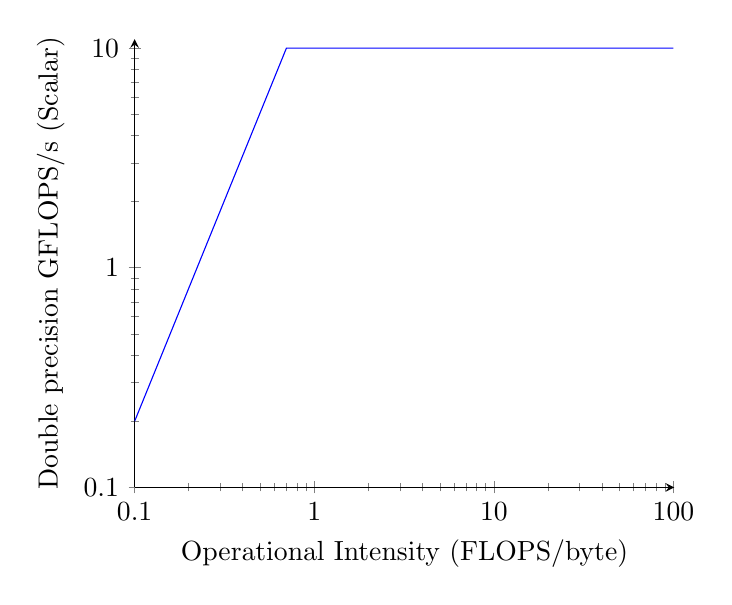
\begin{tikzpicture}
\begin{axis}[
  xmode = log,
  ymode = log,
  axis lines = left,
  xlabel = Operational Intensity (FLOPS/byte),
  ylabel = Double precision GFLOPS/s (Scalar),
  ymin = 0.1,
  xmin = 0.1,
  ymax = 11,
  xmax = 101,
  log ticks with fixed point,
]
\addplot[color=blue] coordinates {
  (0.1, 0.2)
  (0.7, 10)
  (100, 10)
};
\end{axis}
\end{tikzpicture}

\section{Parallel}

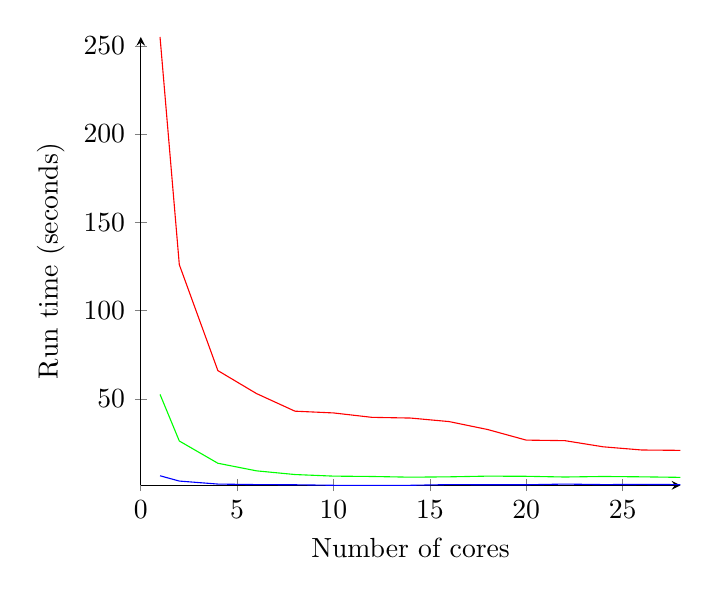
\begin{tikzpicture}
\begin{axis}[
  axis lines = left,
  xlabel = Number of cores,
  ylabel = Run time (seconds),
  xmin = 0,
  ymin = 1,
]
% 128x128
\addplot[color=blue] table {
  1   6.4
  2   3.4
  4   1.7
  6   1.4
  8   1.3
  10  1.0
  12  0.9
  14  1.0
  16  1.4
  18  1.3
  20  1.3
  22  1.7
  24  1.4
  26  1.5
  28  1.4
};

% 256x256 
\addplot[color=green] table {
  1   52.5
  2   26.1
  4   13.5
  6   9.2
  8   7.1
  10  6.2
  12  6.0
  14  5.6
  16  5.8
  18  6.2
  20  6.1
  22  5.7
  24  6.0
  26  5.8
  28  5.5
};

% 1028x1028
\addplot[color=red] table {
  1   255
  2   126
  4   66
  6   53
  8   43 
  10  42
  12  39.5
  14  39.1
  16  37.1
  18  32.6
  20  26.6
  22  26.3
  24  22.8
  26  21.0
  28  20.8
};
\end{axis}
\end{tikzpicture}

\begin{center}
  \begin{tabular}{ |p{1.5cm}||p{1.5cm}|p{1.5cm}|p{1.5cm}| }
 \hline
 \multicolumn{4}{|c|}{Results} \\
 \hline
 Number of cores & 128x128 & 256x256 & 1024x1024 \\
 \hline
 1  & 6.4 &  52.5  &  255     \\
 2  & 3.4 &  26.1  &  126     \\
 4  & 1.7 &  13.5  &  66      \\ 
 6  & 1.4 &  9.2   &  53      \\ 
 8  & 1.3 &  7.1   &  43      \\ 
 10 & 1.0 &  6.2   &  42      \\
 12 & 0.9 &  6.0   &  39.5    \\
 14 & 1.0 &  5.6   &  39.1    \\ 
 16 & 1.4 &  5.8   &  37.1    \\ 
 18 & 1.3 &  6.2   &  32.6    \\
 20 & 1.3 &  6.1   &  26.6    \\
 22 & 1.7 &  5.7   &  26.3    \\ 
 24 & 1.4 &  6.0   &  22.8    \\ 
 26 & 1.5 &  5.8   &  21.0    \\ 
 28 & 1.4 &  5.5   &  20.8    \\
 \hline
\end{tabular}
\captionof{table}{Parallel scaling results from 1-28 cores}
\label{tab:parallelresults}
\end{center}


\end{multicols}
\end{document}

